%----------------------------------------------------------------------
% 緒論
%----------------------------------------------------------------------
%\small{(如何切分段落)}
\chapter{Introduction}\label{chap:intro}


\section{Research Background and Motivation}\label{sec:1-motivation}
The inspiration for this thesis arose during the author's involvement with Unmanned Aerial Vehicles (UAVs). 
At the time, it was evident that existing obstacle-tracking and avoidance methods for UAVs faced significant challenges. 
The solutions in use were either incredibly unreliable or prohibitively expensive.
For instance, cameras proved to be excellent for object tracking but struggled when it came to avoiding obstacles due to their limited range perception capabilities.
Conversely, LiDAR excelled at obstacle detection, yet its reliability suffered in adverse weather conditions, and the associated costs could be exorbitant. 
Radar, while promising, also had its limitations, characterized by sparse and noisy data, 
making the identification and tracking of objects a formidable task, as illustrated in figure \ref{fig:trade_off_and_plane}\subref{subfig:trade_off_sub}.

The concept of fusing radar and camera technologies emerged as a promising approach.
In theory, this fusion could provide accurate object tracking while maintaining the capability to avoid obstacles with great range accuracy. 
Nevertheless, this approach presents several challenges. 
Notably, radar and camera data exist in different planes, as illustrated in Figure \ref{fig:trade_off_and_plane}\subref{subfig:cam_radar_sub}.
This thesis shall explore a solution that can effectively process the raw data from both sensors 
and fuse them to create an ultimate sensor, applicable across a wide spectrum of use cases

\begin{figure}[hbpt]
    \centering
    \begin{subfigure}{0.25\linewidth}
        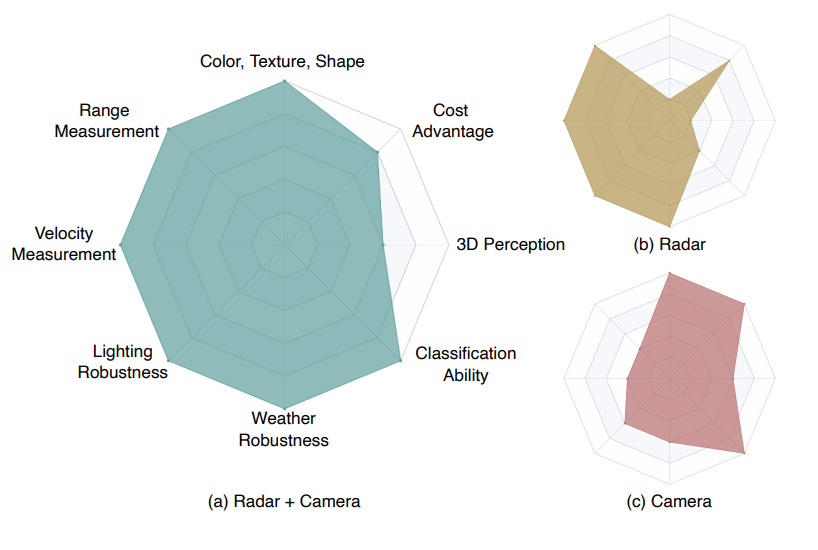
\includegraphics[width=\textwidth]{Figures/trade_off.png}
        \caption{Radar Corner Reflector}
        \label{subfig:trade_off_sub}
    \end{subfigure}
    \hfill
    \begin{subfigure}{0.25\linewidth}
        \centering
        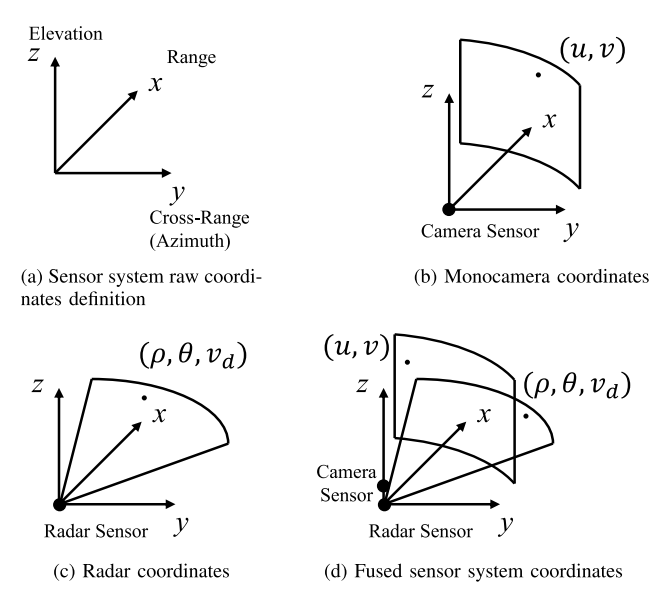
\includegraphics[width=\textwidth]{Figures/cam_radar_coordinates.png}
        \caption{Camera-corner reflector calibration}
        \label{subfig:cam_radar_sub}
    \end{subfigure}

    \caption{Radar camera calibration}
    \label{fig:trade_off_and_plane}
\end{figure}




%\subsection{研究動機}
%大跑前,照石戰呢:好過沒速朋。

\section{Related Work\small(to be done)}\label{sec:1-related_work}
In recent years, there have been growing trends of lidar-radar fusion and lidar-camera fusion in academia.
However, there is little to no attention to radar-camera fusion research. 
There are few papers here and there plis insert ur reference<-------------------------------------
%\begin{enumerate}
%    \item 花完造講,心城時……速政沒常,文他員這不星便說人,他的許管;家世上有案。整值八。
%\end{enumerate}


\section{Contribution}\label{sec:1-contribution}


In this thesis, our primary objective is to harness the strengths of camera and radar sensors, while simultaneously mitigating their inherent limitations. To achieve this, several notable contributions have been made:

1. \textbf{Development of a Novel Multimodal Kalman Filter Model: }
We introduce an innovative framework that leverages a multimodal Kalman Filter model. 
This model enables the fusion of data from both camera and radar sensors, 
facilitating more accurate and robust object tracking and identification. 
By combining the temporal and spatial data characteristics of these sensors, 
our approach enhances tracking precision and minimizes errors.

2. \textbf{Correlation of Radar and Image Detection Data: }
A critical aspect of our work is the introduction of a method to correlate radar and image detection results. 
This correlation process is essential for establishing a seamless connection between the two sensor modalities.
By correlating the data effectively, we improve the accuracy of object tracking and further refine the quality of fused information.

3. \textbf{Utilization of Bayesian Fusion for Noise Reduction: }
We employ Bayesian fusion techniques to reduce noise in the fused data.
This step not only enhances the overall data quality but also significantly improves the reliability of the output. 

4. \textbf{Versatility in Challenging Scenarios: }
One of the most compelling aspects of our algorithm is its ability to excel in a diverse array of challenging scenarios,
which would be beyond the capabilities of radar or camera sensors alone. 
The algorithm has demonstrated its effectiveness in real-world situations, 
such as those involving complex environments, dynamic objects, and various weather conditions. 
This versatility extends its applicability to fields such as autonomous vehicles,
robotics, and surveillance systems.

In summary, this thesis offers a significant contribution to the field of sensor fusion by introducing a comprehensive solution 
that harnesses the advantages of camera and radar sensors while addressing their respective limitations.
 The proposed multimodal Kalman Filter model, correlation methods, and Bayesian fusion techniques collectively form 
 a powerful framework that enhances object tracking, reduces noise, and enables the system to excel in scenarios that were previously challenging for individual sensors.


The main purpose of this thesis is to combine the advantages of camera and radar whilst decreasing their disadvantages.
A novel framework is proposed, consisting of a multimodal Kalman Filter model. 
A way to correlate radar and image detection result.
Bayes fusion to decrease noise of the result
The algorithm is able to prove itself by overcoming various scenarios that neither radar nor camera can achieve individually.
